\documentclass[conference]{IEEEtran}
% \IEEEoverridecommandlockouts
% The preceding line is only needed to identify funding in the first footnote. 
% If that is unneeded, please comment it out.

\usepackage{cite}
\usepackage{amsmath,amssymb,amsfonts}
\usepackage{algorithmic}
\usepackage{graphicx}
\usepackage{textcomp}
\usepackage{xcolor}
\usepackage{url}
\usepackage{listings}
\usepackage{algorithm2e}

% Configure the listings package
\lstset{
    basicstyle=\ttfamily\footnotesize,
    keywordstyle=\color{blue},
    commentstyle=\color{green},
    stringstyle=\color{red},
    numbers=left,
    numberstyle=\tiny\color{gray},
    stepnumber=1,
    numbersep=5pt,
    showspaces=false,
    showstringspaces=false,
    breaklines=true,
    frame=single,
    tabsize=2,
    captionpos=b
}

\def\BibTeX{{\rm B\kern-.05em{\sc i\kern-.025em b}\kern-.08em
    T\kern-.1667em\lower.7ex\hbox{E}\kern-.125emX}}

\begin{document}

\title{Kingdomino: Enter the Virtual World}

\author{\IEEEauthorblockN{Hai Duong, Tran}
    \IEEEauthorblockA{\textit{CSE, Frankfurt University of Applied Sciences} \\
        Frankfurt am Main, Germany \\
        hai.tran2@stud.fra-uas.de}
    \and
    \IEEEauthorblockN{Pham Minh Tuan, Bui}
    \IEEEauthorblockA{\textit{CSE, Frankfurt University of Applied Sciences} \\
        Frankfurt am Main, Germany \\
        pham.bui@stud.fra-uas.de}
}

\maketitle

\begin{abstract}
    This paper presents a digital adaptation of the board game Kingdomino,
    developed using Java and the LibGDX framework. Our implementation leverages an
    event-driven architecture, a flood-fill algorithm for scoring, and shader-based
    rendering to enhance the user experience. We explore key aspects of game logic,
    including tile placement validation, turn-based mechanics, and dynamic UI
    interactions. The paper details the design choices, algorithms, and modular
    structure of the system, ensuring efficiency and scalability. Additionally, we
    evaluate game performance through experimental results and discuss future
    improvements, such as AI integration and multiplayer capabilities.
\end{abstract}

\begin{IEEEkeywords}
    Kingdomino, boardgame, implementation, game development, OOP
\end{IEEEkeywords}

%======================================================
\section{Introduction}
% 1. INTRODUCTION
% -- Explain overall motivation, background, and significance.
% -- Provide a quick overview of the Kingdomino game and the goals of your project.

Kingdomino~\cite{wiki:kingdomino} is a strategic tile placement game where
players act as lords expanding their kingdoms. The objective is to construct
the most prosperous territory by selecting and placing tiles that represent
various terrain types, such as wheat fields, lakes, and mountains. Each tile
comprises two sections that must be connected to the existing kingdom based on
matching terrain types.

A key mechanic in Kingdomino is the tile selection order, which is influenced
by the quality of previous choices. High-value tiles offer strategic benefits
but may result in players selecting tiles later in subsequent rounds,
introducing tactical decision-making. Additionally, tiles with crowns multiply
the value of the connected terrains, significantly impacting the final score.

The game concludes once each player fills their 5$\times$5 grid or can no
longer place tiles. Scoring is determined by the size of connected terrain
groups and the number of crowns they contain. Kingdomino's blend of simple
rules and strategic depth has garnered popularity, making it an excellent
subject for developing and analyzing game-based algorithms.

%======================================================
\section{Problem Description}
% 2. PROBLEM DESCRIPTION
% -- Formal description: definitions, examples.
% -- Description of Kingdomino with examples.

The primary goal in Kingdomino is to construct the most prestigious kingdom by
strategically placing tiles within a constrained 5$\times$5 grid. Players must
explore various terrain types—fields, lakes, mountains, forests, meadows, and
swamps—and connect them to their existing kingdom while adhering to specific
placement rules. Each tile consists of two sections, and at least one section
must match the terrain type of an adjacent tile. Crowns on tiles act as
multipliers to the score of connected terrain groups, encouraging players to
prioritize valuable combinations.

Players compete for tiles through a selection mechanism that balances
high-value tiles with the consequence of selecting later in subsequent rounds.
This creates an optimization problem where players must maximize immediate
gains while strategically positioning themselves for future moves. The game
concludes when each player has filled their grid or can no longer place tiles,
with scoring determining the winner based on terrain connectivity and crown
placements.

\begin{figure*}[htbp]
    \centerline{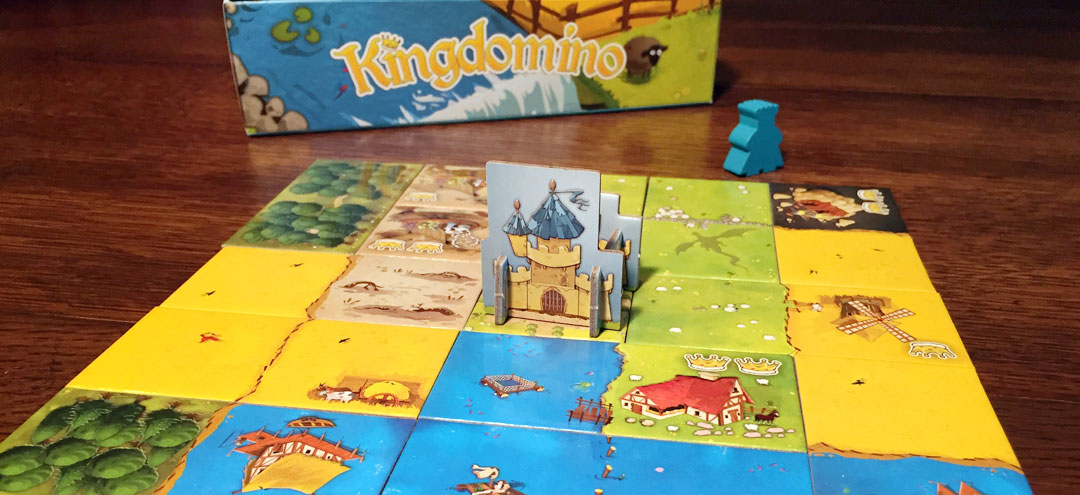
\includegraphics[width=\textwidth]{assets/kingdomino.jpg}}
    \caption{Kingdomino Board Game.}\label{fig:kingdomino}
\end{figure*}

\subsection{Formal Description}

The game involves the following components and constraints:

\subsubsection{Components}

\begin{itemize}
    \item \textbf{Tiles}: Each tile consists of two sections, each representing one of the six terrain types (fields, lakes, mountains, forests, meadows, and swamps). Certain tiles include crowns, which serve as score multipliers.
    \item \textbf{Kingdom}: A 5$\times$5 grid where tiles are placed. Each player starts with a central tile (wild type) and builds outward.
    \item \textbf{Selection Order}: Players select tiles in descending order of tile value (higher numbers first) and use their selection to determine the order in subsequent rounds.
\end{itemize}

\subsubsection{Rules}

\begin{itemize}
    \item \textbf{Placement}:
          \begin{itemize}
              \item Tiles must connect to at least one adjacent tile with the same terrain type
                    (horizontally or vertically).
              \item The grid is limited to 5$\times$5 dimensions; any tile that cannot be placed is
                    discarded.
          \end{itemize}

    \item \textbf{Scoring}:
          \begin{itemize}
              \item Points are calculated as the product of the number of connected tiles of the
                    same terrain and the number of crowns within the connected group.
              \item Bonuses include:
                    \begin{itemize}
                        \item +10 points for placing the central castle at the grid's center.
                        \item +5 points for completing a full grid.
                    \end{itemize}
          \end{itemize}

    \item \textbf{Game Variants}:
          \begin{itemize}
              \item A 7$\times$7 grid variant for advanced play.
              \item Multi-round gameplay (Dynasty mode) with cumulative scores.
          \end{itemize}
\end{itemize}

\subsubsection{Objective}

Maximize the total score by constructing a kingdom that balances large
connected terrain groups with crown placements, while competing against other
players for optimal tile selection.

\subsection{Examples of Gameplay}
% -- Provide short examples or scenarios that clarify the rules.

Gameplay is explain in Appendix~\ref{app:gameplay}.

%======================================================
\section{Related Work}
% 3. RELATED WORK
% -- Discuss any algorithms or approaches that are relevant, 
%    e.g., fractals, data generation, evolutionary algorithms, etc.
% -- Mention similar or existing board games / AI approaches.
Board games like Carcassonne\cite{wiki:carcassonne} and
Patchwork\cite{wiki:patchwork} offer valuable insights into the mechanics of
tile placement and scoring, making them relevant to our implementation of
Kingdomino. Carcassonne challenges players to build cities, roads, and fields
by placing tiles based on terrain type, a mechanic that closely aligns with
Kingdomino’s terrain-matching rules. Similarly, Patchwork emphasizes the
efficient use of a constrained grid, much like Kingdomino’s 5×5 board, where
players must optimize placement for maximum scoring. These games demonstrate
how simple mechanics can result in complex decision-making, a feature we aim to
replicate in our project.

In addition to inspiration from traditional board games, the implementation of
Kingdomino leverages several key computational and architectural techniques.
The scoring mechanism, for instance, utilizes a flood-fill
algorithm\cite{wiki:floodfill} to evaluate the connected terrain groups and
their associated scores. This algorithm, commonly employed in image processing
and graph traversal\cite{wiki:graphtraversal}, provides an efficient way to
traverse and calculate properties of contiguous regions. Its application in
Kingdomino ensures accurate and performant scoring calculations, even as the
board becomes increasingly complex during gameplay.

The game is designed using an event-driven architecture\cite{wiki:eventdriven,
    wiki:floodfill}, where interactions, where interactions such as tile placement
and scoring updates are managed asynchronously through an EventManager. This
approach is prevalent in modern game frameworks and engines, such as LibGDX,
Unity, and Unreal Engine, and ensures a clear separation between game logic and
user input. By decoupling these components, the design achieves improved
modularity and scalability, enabling future enhancements such as AI integration
or multiplayer features. The intention was to implement Entity-Component-System
(ECS) architecture\cite{wiki:ecs} to further improve the game's performance and
scalability. But we not strictly follow this architecture for flexibility and
simplicity.

Furthermore, the aesthetic design of Kingdomino draws from pixel-art-inspired
games, including Balatro\cite{wiki:balatro}, which use vibrant colors and
minimalistic textures to create a visually engaging experience. This style has
been adopted to maintain the simplicity of the board game while enhancing the
digital adaptation with a modern and nostalgic visual appeal.

Finally, the use of the LibGDX framework\cite{libgdx} streamlines development,
particularly in rendering, asset management, and input handling. By leveraging
tools such as TextureAtlas\cite{wiki:textureatlas} for managing game assets and
InputMultiplexer for handling player interactions, the framework supports an
efficient implementation of Kingdomino's mechanics and aesthetics. This
integration aligns with industry-standard practices for creating scalable,
interactive applications.

Incorporating these approaches and inspirations, the implementation of
Kingdomino aims to balance simplicity, efficiency, and engagement, ensuring a
faithful and enjoyable digital representation of the original board game.

% Example referencing
% As noted by some authors \cite{exampleRef1}, 
% board games have often been used to benchmark AI approaches.

%======================================================
\section{Teamwork}
% 4. TEAMWORK
% -- Who did what, how the tasks were divided, how you communicated and tracked progress, 
%    brainstorming sessions, etc.

\begin{figure*}[htbp]
    \centerline{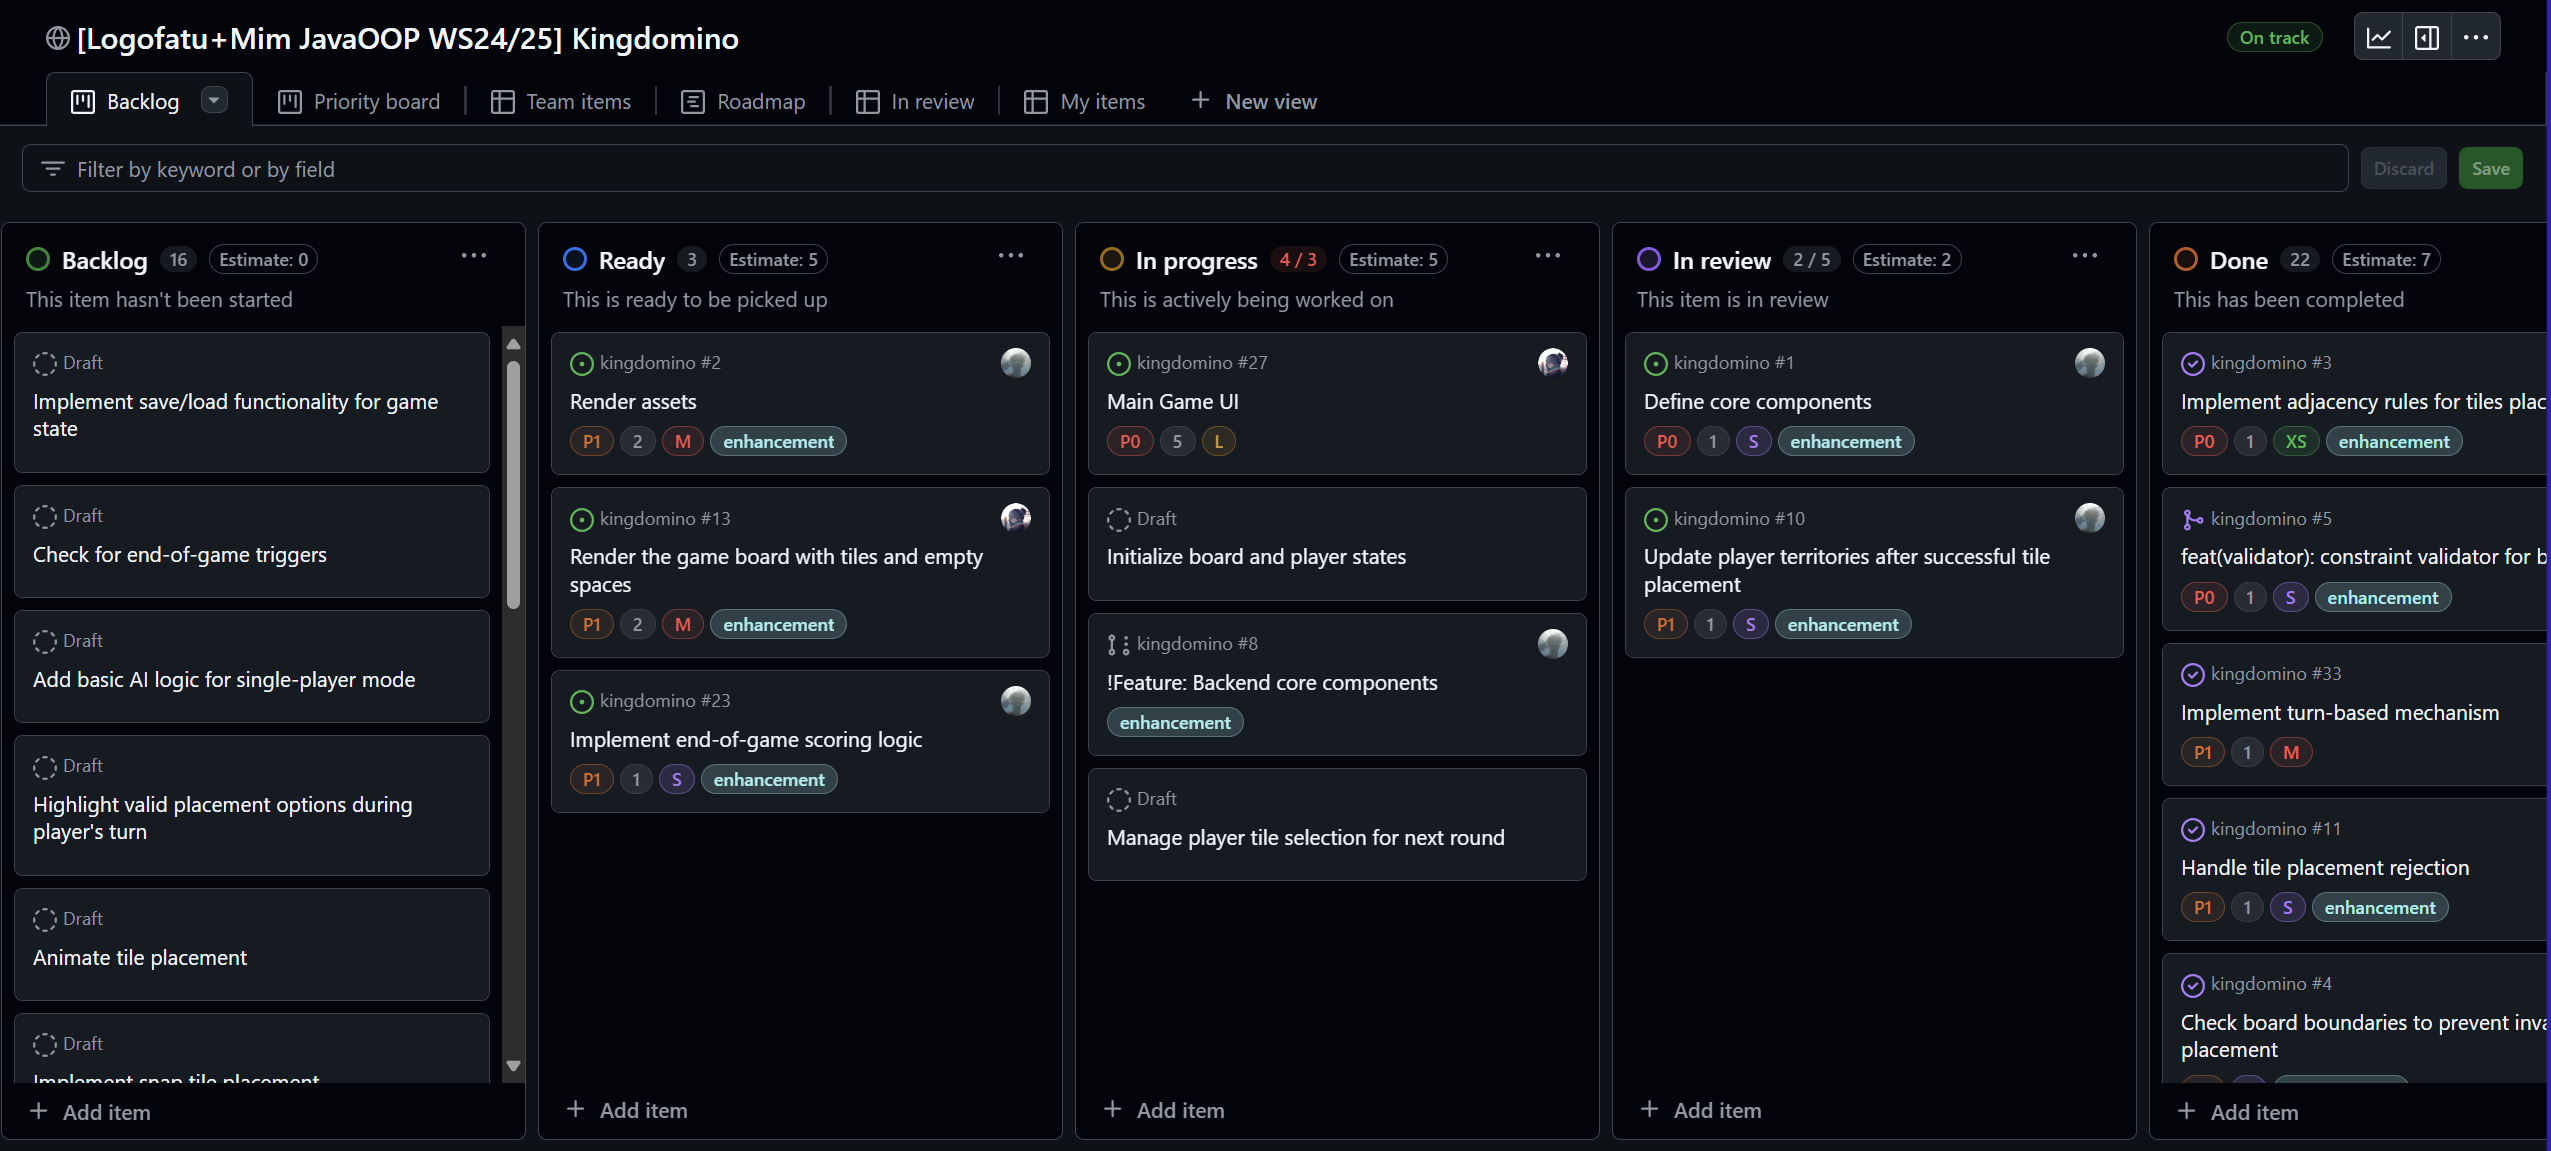
\includegraphics[width=0.8\textwidth]{assets/github-project.png}}
    \caption{Kanban Board implements SCRUM planning technique.}\label{fig:kanban}
\end{figure*}

In general, the project was divided into two main parts: the game logic and the
graphical user interface (GUI). We used GitHub Project to track and communicate
with each other.

We ultilize SCRUM (Fig~\ref{fig:kanban}) methodology to manage our project. For
more details, see the GitHub Project board.

\subsection{Roles and Responsibilities}
% -- Person A, Person B
For the game logic, Hai Duong Tran was responsible for almost all backend logic
including the implementation of the tile placement rules, scoring mechanism,
and the overall game flow. He also integrated the flood-fill algorithm for
scoring and ensured the game logic adhered to the official Kingdomino rules.
Moreover, he worked on shader to add an extra visual effect to the game.

Pham Minh Tuan Bui focused on the graphical user interface (GUI) and user
interactions. He designed the layout, managed the rendering of game elements
using the LibGDX framework, and implemented the event-driven architecture to
handle user inputs and game state updates. Additionally, he worked on the
visual aesthetics and ensured a smooth user experience.

Even though we had our own responsibilities, we often collaborated on various
aspects of the project. We held regular meetings to discuss progress,
brainstorm solutions to challenges, and ensure that our work was aligned. Code
reviews were conducted to maintain quality and consistency, and we frequently
pair-programmed to tackle complex problems together. This collaborative
approach not only enhanced our productivity but also fostered a deeper
understanding of the project as a whole.

\subsection{Collaboration Tools and Workflow}
% -- Bug tracking, repository management, code reviews, etc.

We mainly use GitHub Issues and Pull Requests to track bugs and feature
requests. Each team member created branches for their respective tasks,
ensuring that the main branch remained stable.

Moreover, we practice code review through GitHub Pull
Requests\ref{fig:github-pr}. This ensures that all code changes are reviewed by
other team member before being merged into the main branch. This process helps
to maintain code quality, catch potential bugs early, and facilitate knowledge
sharing among team members. Each pull request includes a description of the
changes, and reviewers provide feedback, request modifications, or approve the
changes. This collaborative approach to code review has been instrumental in
maintaining a high standard of code throughout the project.

\begin{figure}[htbp]
    \centerline{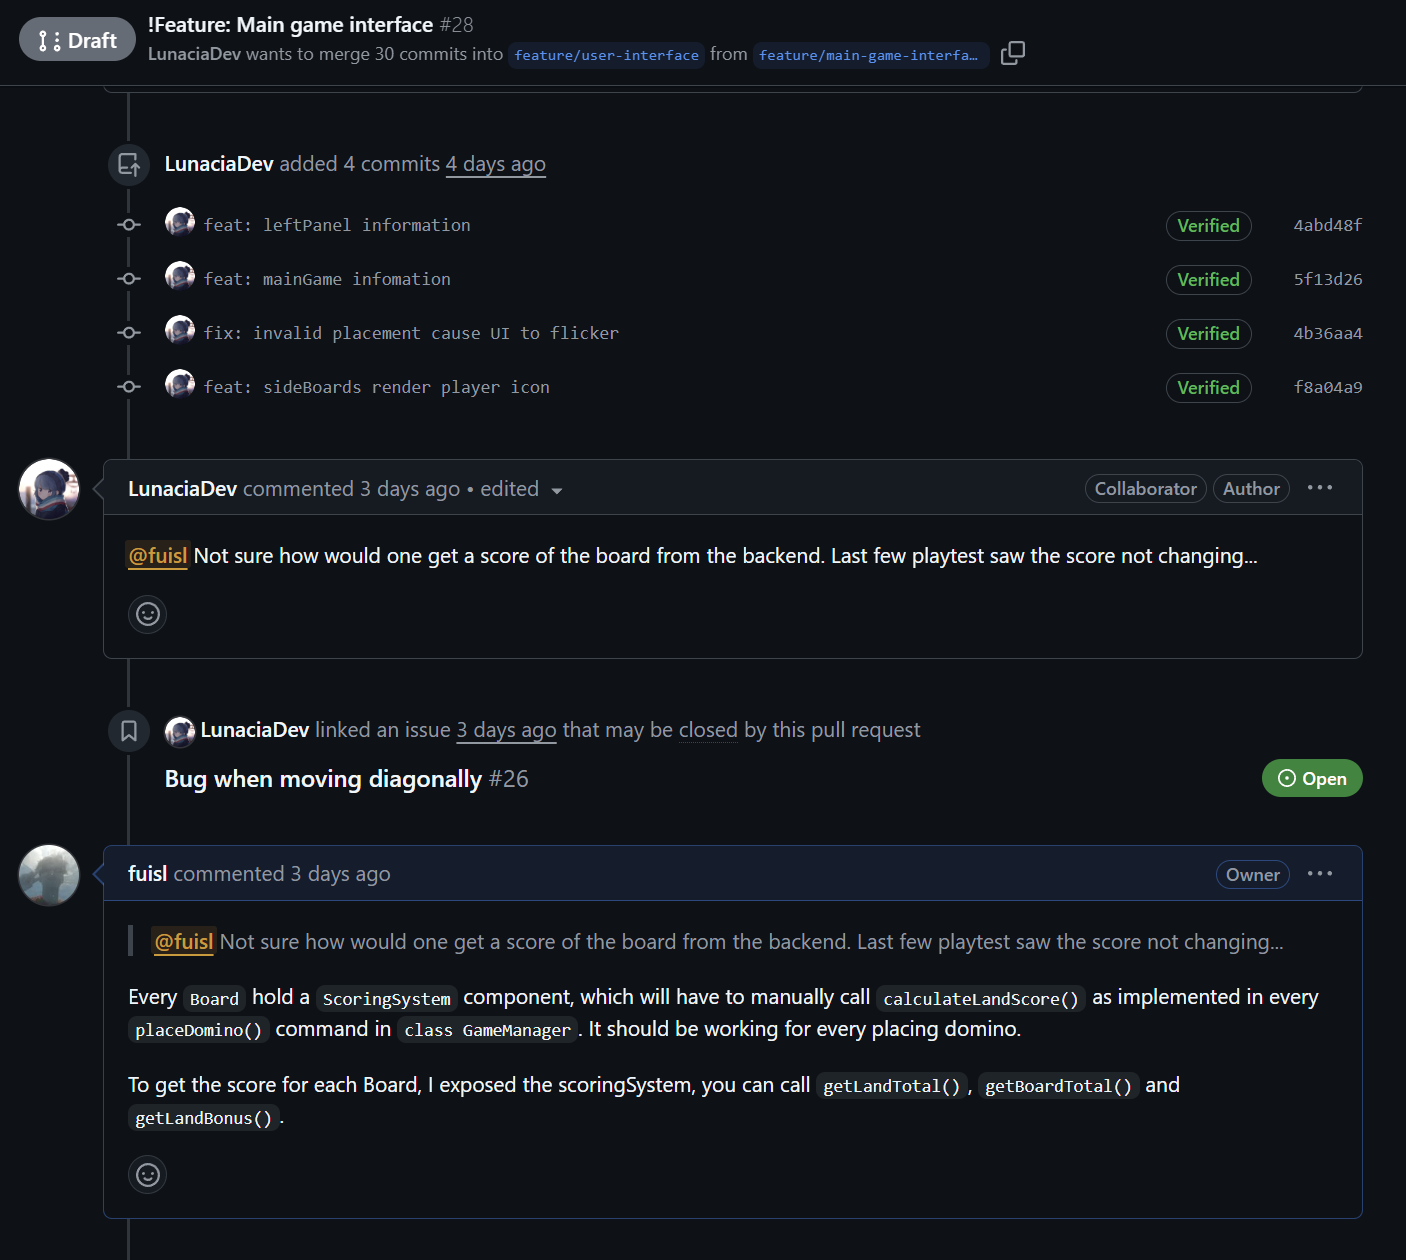
\includegraphics[width=0.48\textwidth]{assets/github-pr.png}}
    \caption{A conversation in one Pull Request.}\label{fig:github-pr}
\end{figure}

For communication, we relied on Messenger for real-time discussions and meet
each other at school or guest house for meetings. We documented our progress
and decisions via commit messages. Other document which included meeting notes,
design documents, and brainstorming sessions are stored in the form of digital
draft. This collaborative approach ensured transparency and kept everyone
aligned with the project's goals.

%======================================================
\section{Proposed Approaches}
% 5. PROPOSED APPROACHES
% -- Input/Output technique.
% -- Algorithm/Pseudocode.
% -- Process flow diagram (if necessary).
% summary of the section

\subsection{Event-Driven Architecture}
% -- Explanation of the event-driven architecture, how is it involved in the game.

Kingdomino’s digital adaptation uses an event-driven architecture to manage
user interactions, game state transitions, and visual effects efficiently. This
approach decouples game logic, input handling, and rendering, improving
performance, modularity, and maintainability.

\subsection{Core Components}
\subsubsection{Event Class}
The \texttt{Event} class encapsulates actions that can be executed immediately
or after a delay. It supports different types of triggers:
\begin{itemize}
    \item \textbf{IMMEDIATE}: Executes the event as soon as it is created.
    \item \textbf{BEFORE}: Executes an action and then enforces a delay before completing.
    \item \textbf{AFTER}: Executes an action only after a specified delay.
    \item \textbf{CONDITION}: Executes when a certain condition is met.
    \item \textbf{EASE}: Implements smooth transitions for visual effects.
\end{itemize}
Each event has attributes such as blocking, blockable, complete, and delay, allowing for controlled execution within the game loop.

\subsubsection{EventManager}
The \texttt{EventManager} acts as the central execution hub for all
game-related events. It maintains multiple concurrent event queues, categorized
into:
\begin{itemize}
    \item \textbf{Base}: Core gameplay logic (e.g., turn transitions, score updates).
    \item \textbf{Input}: Player interactions (e.g., movement, rotation, placement).
    \item \textbf{Background}: Visual effects and animations.
    \item \textbf{Sound}: Audio effects (e.g., movement, tile placement, invalid moves).
    \item \textbf{Other}: Miscellaneous actions.
\end{itemize}
The event manager ensures concurrency safety using \texttt{ConcurrentLinkedQueue}, preventing race conditions when processing multiple asynchronous actions.

\subsubsection{GameTimer}
The \texttt{GameTimer} class tracks real-time, total elapsed time, and
background animation timing. It synchronizes event execution by accumulating
delta time (dt) and updating event processing intervals accordingly. The timer
provides a consistent timing reference for executing delayed events and easing
functions.

\subsubsection{Ease}
The \texttt{Ease} class facilitates smooth animations for background effects,
screen transitions, and UI enhancements. It supports different interpolation
methods:
\begin{itemize}
    \item \textbf{LERP (Linear Interpolation)}: Gradually changes a value over time.
    \item \textbf{ELASTIC}: Simulates spring-like motion for dynamic effects.
    \item \textbf{QUAD}: Creates a smooth acceleration effect.
\end{itemize}
This is particularly useful for animations such as screen shaking when an invalid move is made, or color transitions when switching player turns.

\subsection{Input Handling}
Kingdomino implements manual input event processing instead of relying on
LibGDX’s built-in event loop. The \texttt{BoardInputHandler} class captures
user input and translates it into structured events.

\subsubsection{Key Features of Input Handling}
\begin{itemize}
    \item \textbf{Deferred Execution}: Input actions are queued and processed asynchronously.
    \item \textbf{State-Based Processing}: Input is processed only in relevant game states.
    \item \textbf{Feedback Integration}: Invalid actions trigger audio and visual feedback.
\end{itemize}

\subsubsection{Example: Handling Movement Events}
When a player moves a domino using the keyboard or controller:
\begin{enumerate}
    \item Input is captured (WASD keys or joystick).
    \item \texttt{BoardInputHandler} checks validity (e.g., ensuring the move is within bounds).
    \item If valid, an event is created and queued:
          \begin{lstlisting}[language=Java]
Event moveEvent = new Event(
    TriggerType.BEFORE, true, true, 0.15f, // Delay for smooth input
    () -> currentDomino.moveDomino(Direction.UP),
    null, null, null);
eventManager.addEvent(moveEvent, "input", false);
    \end{lstlisting}
    \item The event executes smoothly without blocking the main loop.
    \item If the move is invalid, audio and visual feedback are triggered:
          \begin{lstlisting}[language=Java]
audioManager.playSound(AudioManager.SoundType.CANCEL);
BackgroundManager.screenShake();
    \end{lstlisting}
\end{enumerate}
This approach ensures efficient, responsive, and user-friendly interactions.

\subsection{Benefits}
\begin{itemize}
    \item \textbf{Improved Responsiveness}: Actions are processed only when necessary, reducing redundant calculations.
    \item \textbf{Modularity and Scalability}: New game mechanics (e.g., AI, online multiplayer) can be easily integrated as event handlers.
    \item \textbf{Concurrency and Performance Optimization}: Parallel event queues prevent input lag and improve game fluidity.
\end{itemize}

%======================================================
\section{Implementation Details}
% 6. IMPLEMENTATION DETAILS
% -- Application structure, GUI details, UML/Class Diagram, used libraries, important code snippets.

\subsection{Game States}

In the implementation of Kingdomino, the game progresses through a series of
well-defined states. Each state represents a distinct phase of the game,
ensuring a structured flow from the beginning to the end. The primary game
states include:

\begin{itemize}
    \item \textbf{Init}: The initial state where the game components are set up and initialized.
    \item \textbf{Setup}: This state involves preparing the game board, shuffling tiles, and setting up players for the game.
    \item \textbf{Turn Start}: Marks the beginning of a player's turn, where the current player and available tiles are determined.
    \item \textbf{Turn Placing}: The state where the player places their selected tile on the board according to the game rules.
    \item \textbf{Turn Choosing}: The state where the player selects a tile for the next round.
    \item \textbf{Turn End}: Concludes the current player's turn and transitions to the next player.
    \item \textbf{Game Over}: The final state when the game ends, and no more moves can be made.
    \item \textbf{Results}: Displays the final scores and determines the winner based on the game rules.
\end{itemize}

Each state transitions to the next based on player actions and game logic. The
following diagram illustrates the state transitions:

\begin{figure}[htbp]
    \centerline{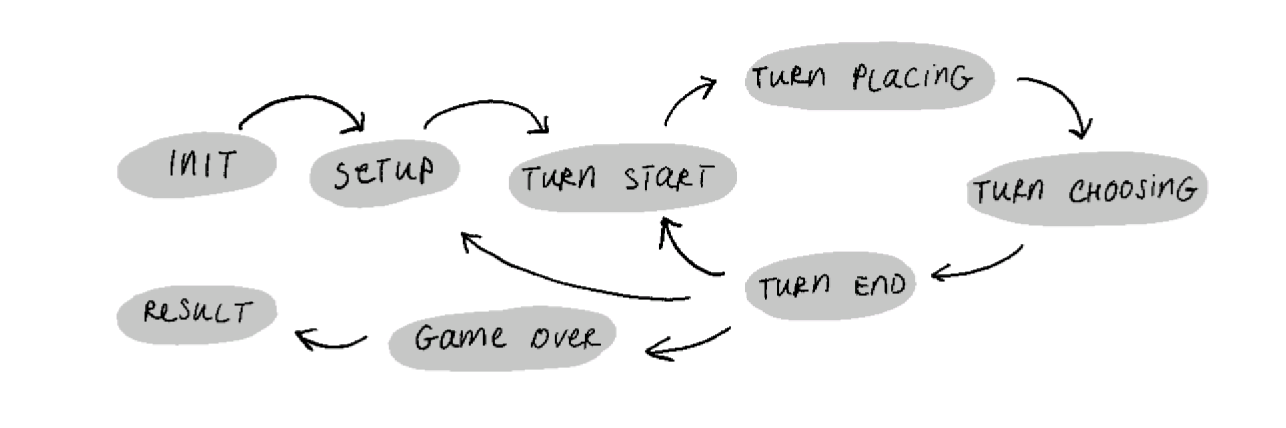
\includegraphics[width=0.55\textwidth]{assets/states.png}}
    \caption{Game State Transitions.}\label{fig:game_states}
\end{figure}

\subsection{Game Units and High-Level Architecture}
% -- High-level architecture. Possibly a diagram.

Tile is the essential, smallest accessible unit for this game. Tile holds 2
most important attributes: TerrainType and Number of Crowns.

\begin{figure}[htbp]
    \centerline{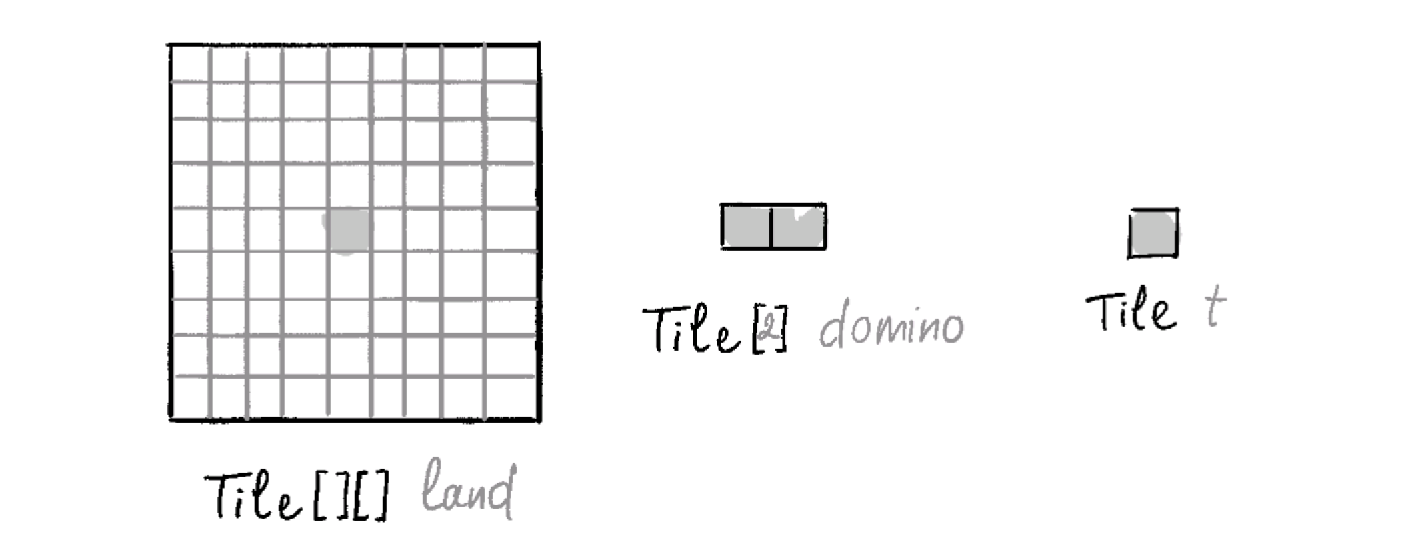
\includegraphics[width=0.48\textwidth]{assets/unit.png}}
    \caption{Units of Tile.}\label{fig:unit}
\end{figure}

Board is 2-dimensional array of type Tile. Though Board has more attributes and
methods which supports interactions between GameManager and Board, Tile[][] is
where Tiles being store and perform logic on.

On the other hand, Domino is an interface between human player and Board. It
holds informations about location, validator, etc., which related to action
that can be performed on Board (like moving, rotating or placing Domino). The
actual Domino will not be placed in Board, only the two Tiles that composes
Domino would be added. Domino will then be discarded.

\subsection{Tile Placement and Board Validation}

\subsubsection{Domino and DominoController}

The \texttt{Domino} class represents a domino in the game, consisting of two
tiles and a controller. It provides methods to rotate, move, and set the
position of the domino. The \texttt{DominoController} class handles the
rotation and placement of dominos, maintaining the state of the tiles and their
positions.

\begin{figure}[htbp]
    \centerline{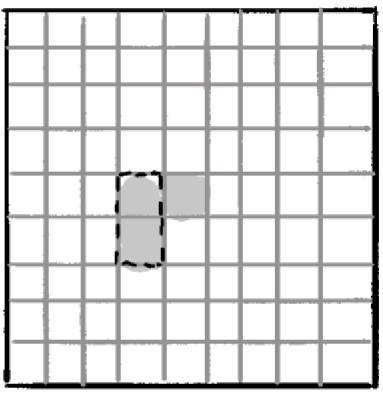
\includegraphics[width=0.18\textwidth]{assets/placing-1.png}}
    \centerline{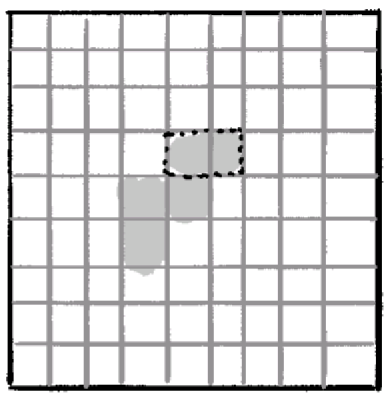
\includegraphics[width=0.18\textwidth]{assets/placing-2.png}}
    \caption{Placing Domino.}\label{fig:placing}
\end{figure}

\begin{lstlisting}[language=Java]
// filepath: /e:/projects/kingdomino/core/src/main/java/dev/kingdomino/game/Domino.java
public class Domino {
    // ...existing code...
    public void rotateDomino(boolean clockwise, boolean shouldOffset) {
        dominoController.rotateDomino(clockwise, shouldOffset);
    }
    // ...existing code...
}
\end{lstlisting}

\begin{lstlisting}[language=Java]
// filepath: /e:/projects/kingdomino/core/src/main/java/dev/kingdomino/game/DominoController.java
public class DominoController {
    // ...existing code...
    public void rotateDomino(boolean clockwise, boolean shouldOffset) {
        lastRotationIndex = rotationIndex;
        rotationIndex = (rotationIndex + (clockwise ? 1 : 3)) % 4;

        // rotate the 2nd Tile with 1st Tile as center
        tileRotator.rotate(posTileA, posTileB, rotationIndex, shouldOffset);

        lastAction = 1;
    }
    // ...existing code...
}
\end{lstlisting}

\subsubsection{TileRotator}

The \texttt{TileRotator} class is responsible for rotating tiles around a
center position. It uses a predefined set of directions to determine the new
position of the tile after rotation.

\begin{figure}[htbp]
    \centerline{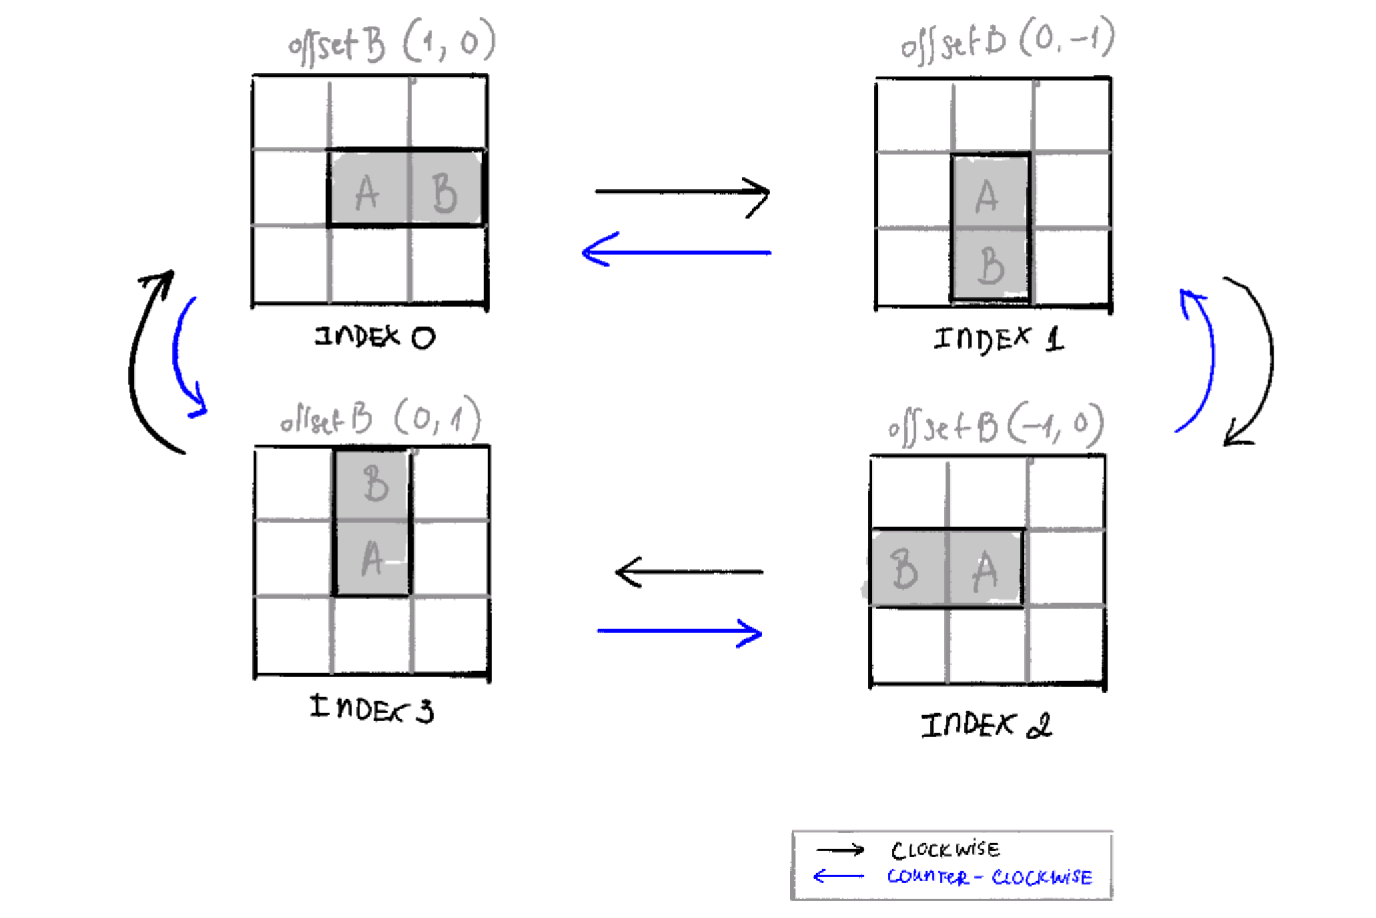
\includegraphics[width=0.55\textwidth]{assets/rotate.png}}
    \caption{Rotate Domino by moving TileB relative to TileA.}\label{fig:rotate}
\end{figure}

The rotation logic for the domino can be described as follows:

\[
    \text{If rotating clockwise:} \quad\boxed{\text{index} = (\text{index} + 1) \mod 4}
\]
\[
    \text{If rotating counter-clockwise:} \quad\boxed{\text{index} = (\text{index} + 3) \mod 4}
\]

\begin{lstlisting}[language=Java]
// filepath: /e:/projects/kingdomino/core/src/main/java/dev/kingdomino/game/TileRotator.java
public class TileRotator {
    // ...existing code...
    public void rotate(Position center, Position tilePos, int rotationIndex, boolean shouldOffset) {
        Position newPos = center.add(directions[rotationIndex]);
        tilePos.set(newPos);
    }
    // ...existing code...
}
\end{lstlisting}

\subsubsection{Tile Placement Validation}

The \texttt{TileValidator} class is responsible for validating the placement of
tiles on the game board. It ensures that tiles are placed within bounds and are
free from occupation. The following code snippet shows the implementation of
the \texttt{TileValidator} class:

\begin{lstlisting}[language=Java]
// filepath: /e:/projects/kingdomino/core/src/main/java/dev/kingdomino/game/TileValidator.java
public class TileValidator {
    // ...existing code...
    public boolean isTilePlaceable(Tile tile, int x, int y) {
        return isTileFree(x, y) && isTileWithinBound(x, y);
    }
    // ...existing code...
    public boolean isTileWithinBound(int x, int y) {
        if (x < minX || x > maxX) {
            if (abs(x - minX) + 1 > size || abs(x - maxX) + 1 > size) {
                return false;
            }
        }
        if (y < minY || y > maxY) {
            if (abs(y - minY) + 1 > size || abs(y - maxY) + 1 > size) {
                return false;
            }
        }
        return true;
    }
    // ...existing code...
    public boolean isTileFree(int x, int y) {
        if (isTileWithinLand(x, y)) {
            return land[y][x] == null;
        }
        return false;
    }
    // ...existing code...
}
\end{lstlisting}

\subsection{Scoring Mechanism}
% -- Explain the flood-fill algorithm and its application in Kingdomino.

The flood-fill algorithm is a computer graphics algorithm used to determine the
area connected to a given node in a multi-dimensional array. It is commonly
used in tools like paint bucket in graphics editors to fill bounded areas with
color.

In the context of Kingdomino, the flood-fill algorithm is utilized to calculate
the score by identifying and evaluating connected groups of the same terrain
type. The algorithm traverses the game board, starting from a given tile, and
recursively explores all adjacent tiles of the same terrain type. This allows
the game to efficiently compute the size of each connected terrain group and
apply the scoring rules based on the number of crowns within these groups.

Below is a pseudocode representation of the recursive 4-way flood-fill
algorithm:

\begin{algorithm}[htbp]
    \caption{Flood-fill Algorithm}
    \KwIn{Tile}
    \KwOut{Flood-filled region}
    \If{Tile is not inside Region}{
        \Return\;
    }
    Set the node\;
    Perform Flood-fill one step to the south of Tile\;
    Perform Flood-fill one step to the north of Tile\;
    Perform Flood-fill one step to the west of Tile\;
    Perform Flood-fill one step to the east of Tile\;
    \Return\;
\end{algorithm}

This algorithm is in its original form. For Kingdomino with multiplicative
scoring system, we need to modify the algorithm to calculate both the spanned
region (area) and also count the number of crowns within the connected group.
See Listing~\ref{lst:floodfill} for the implementation details.

To better illustrate the concept of flood-fill, consider the following example
with a 9$\times$9 grid:

\begin{figure}[htbp]
    \centerline{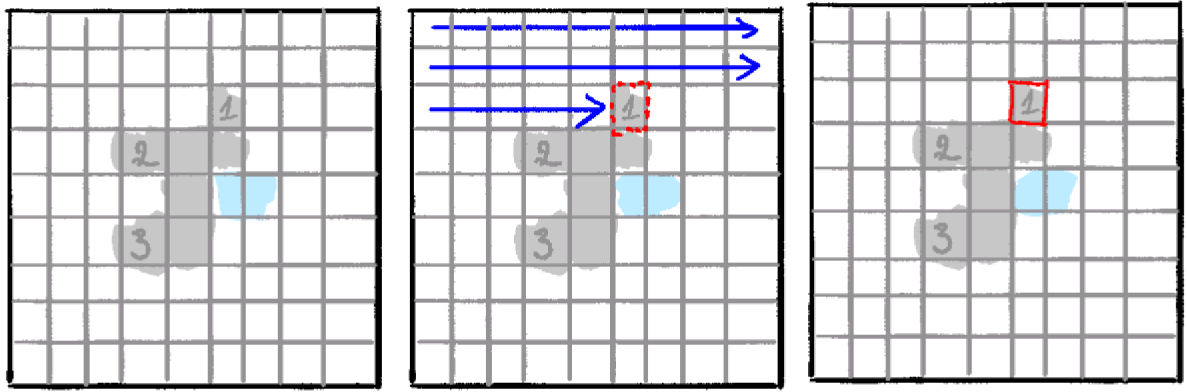
\includegraphics[width=0.48\textwidth]{assets/floodfill-start.png}}
    \centerline{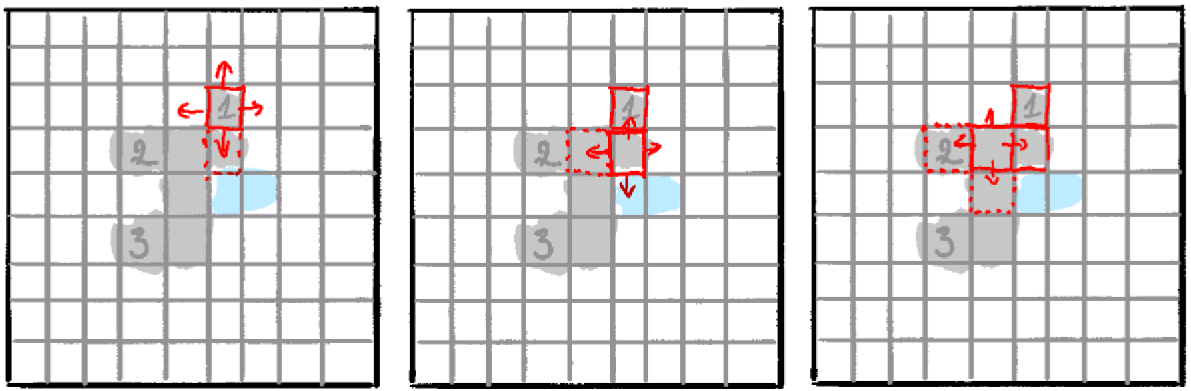
\includegraphics[width=0.48\textwidth]{assets/floodfill-detected.png}}
    \centerline{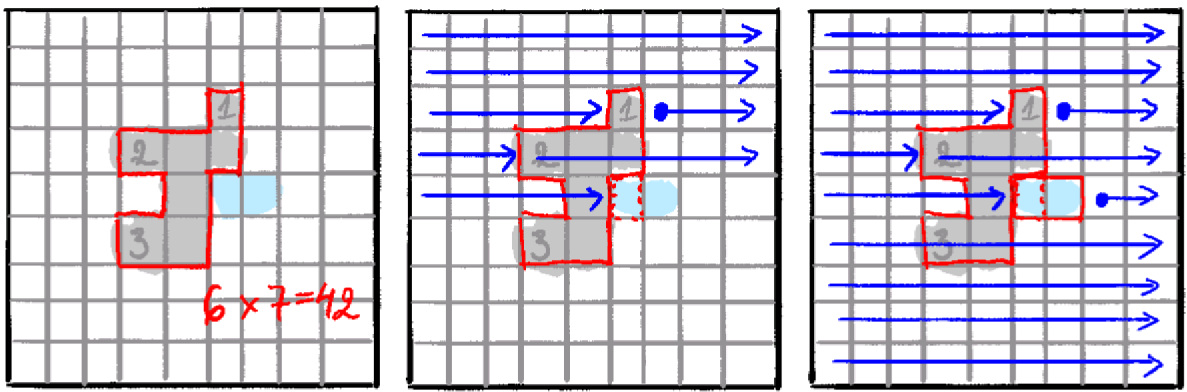
\includegraphics[width=0.48\textwidth]{assets/floodfill-continue.png}}
    % \caption{}\label{fig:floodfill-start}
\end{figure}

In this example, the algorithm starts at the selected tile (highlighted in
red). It then recursively explores all adjacent tiles of the same terrain type,
marking them as visited and counting the number of crowns within the connected
group. The process continues until all connected tiles of the same terrain type
have been evaluated, resulting in the final score for that terrain group.

\subsection{Input Handling}
% -- Describe how user inputs are processed and handled (keyboard and controller).

\subsubsection{Board Navigation}

\subsubsection{Domino Selection}

\subsection{UML/Class Diagram}
% -- Provide an overview of classes, relationships. 
%    Reference the figure in text.

\subsection{Used Libraries and Environment}
% -- Mention languages, frameworks, libraries, operating systems, version details, etc.

\subsection{Important Code Snippets}
% -- Show the relevant or tricky parts of your code with explanations.

\begin{lstlisting}[language=Java, caption={Flood-Fill Algorithm}, label={lst:floodfill}]
private int floodFill(int x, int y, TerrainType terrain, boolean[][] visited) {
    if (x < 0 || x >= land.length || y < 0 || y >= land.length) {
        return 0;
    }

    if (land[y][x] == null || visited[y][x] || land[y][x].getTerrain() != terrain) {
        return 0;
    }
    

    totalCrown += land[y][x].getCrown();
    visited[y][x] = true;

    return 1 +
            floodFill(x + 1, y, terrain, visited) +
            floodFill(x - 1, y, terrain, visited) +
            floodFill(x, y + 1, terrain, visited) +
            floodFill(x, y - 1, terrain, visited);
    }
\end{lstlisting}

%======================================================
% -- mainly UI

\section{Graphical Enhancement and Visual Effects}
% -- Describe the interface design, layout, main widgets.

\subsection{Shader-Based Rendering}
Kingdomino leverages shader-based rendering using OpenGL Shader language to
enhance visual effects and provide a more immersive experience. Two primary
shaders are used: the CRT shader and the background shader.

\subsubsection{CRT Shader}
The CRT shader simulates the appearance of an old CRT monitor, adding effects
such as distortion, scanlines, noise, and bloom. It consists of a vertex shader
and a fragment shader.

\begin{itemize}
    \item \textbf{Vertex Shader (crt.vert)}: Applies transformations to simulate a parallax effect based on mouse position and screen scale.
    \item \textbf{Fragment Shader (crt.frag)}: Implements various visual effects, including barrel distortion, edge feathering, glitch offsets, chromatic aberration, scanlines, and noise overlay.
\end{itemize}

\subsubsection{Background Shader}
The background shader creates dynamic and visually appealing backgrounds with
effects like spinning and color transitions.

\begin{itemize}
    \item \textbf{Vertex Shader (background.vert)}: Passes texture coordinates to the fragment shader.
    \item \textbf{Fragment Shader (background.frag)}: Applies pixelation, swirl, and paint effects based on time and spin parameters, along with color blending for a vibrant background.
\end{itemize}

\subsection{Dynamic UI Elements}
% ...existing code...

\subsection{Background Shader}
% ...existing code...

\subsection{CRT Shader Overlay}
% ...existing code...

\subsection{Visual and Effects}
% ...existing code...

%======================================================
\section{Experimental Results}
% 7. EXPERIMENTAL RESULTS, STATISTICAL TESTS, RUNNING SCENARIOS
% -- Provide tables, charts, and discussion of the experiments you ran.

\subsection{Performance Analysis}
% -- Discuss the performance of the game, any bottlenecks, optimizations.
framerate, input lag event-driven vs. sync update

\subsection{Correctness and Scalability}
% -- Describe your environment, parameter choices, etc.

\subsection{UI/Gameplay Smoothness}
% -- Insert tables and charts with relevant data and evaluations.

% \begin{table}[htbp]
% \caption{Example of Results Table}
% \begin{center}
% \begin{tabular}{|c|c|c|}
% \hline
% \textbf{Parameter} & \textbf{Value / Range} & \textbf{Observation}\\
% \hline
% Population Size & 50--200 & Performance improved \\
% Mutation Rate   & 5\%     & Minimal difference \\
% \hline
% \end{tabular}
% \label{tab:results}
% \end{center}
% \end{table}

%======================================================
\section{Conclusions and Future Work}
% 8. CONCLUSIONS AND FUTURE WORK
% -- Discuss overall findings, reflect on teamwork, 
%    lessons learned, and possible future improvements.

Lorem ipsum dolor sit amet, consectetur adipiscing elit.

\subsection{What We Learned}
% -- Key lessons from implementing or analyzing the game.

\subsection{Future Development}
% -- Potential expansions, new game modes, new algorithms, etc.

%======================================================
\appendices%
\section{Gameplay Mechanic}\label{app:gameplay}
% -- Provide additional content that supports the main text.

%======================================================
% -- Follow the IEEE reference style
% -- Cite references in text, e.g., [1], [2], etc.

\bibliographystyle{IEEEtran}
\bibliography{bibliography}

\end{document}
